\section{Overview}

The NTU HPC cluster, located at Parallel and Distributed System Lab (PDSL), is managed and used by the NTU HPC team\footnote{http://ntuhpc.org}. Its main purpose is for members of NTU HPC to get hands-on skills on optimizing applications for supercomputers and practice applications used in student cluster competitions.

\subsection{Cluster architecture}

The cluster consists of 4 nodes. There are 2 CPU nodes and 2 GPU nodes. The nodes are connected with 1Gbit/s Ethernet. Amongs the nodes, only compute0 is connected to NTU's network. The detailed specification for both CPU and GPU nodes are shown in Table \ref{table:cpu} and Table \ref{table:gpu}.

\begin{table}[ht]
\centering
\caption{CPU node specification}
\label{table:cpu}
\begin{tabular}{|l|l|}
\hline
\textbf{Nodes}      & compute0, compute1                       \\ \hline
\textbf{CPU}        & Intel X5660 (6 cores, 2.8GHz, HT, Turbo) x 2 \\ \hline
\textbf{Memory}     & DDR3 32GB                                \\ \hline
\textbf{Hard drive} & 480GB SATA HDD                           \\ \hline
\textbf{Network}    & 1Gbit/s Ethernet                         \\ \hline
\textbf{Operating system} & CentOS 7.2                         \\ \hline
\end{tabular}
\end{table}

\begin{table}[ht]
\centering
\caption{GPU node specification}
\label{table:gpu}
\begin{tabular}{|l|l|}
\hline
\textbf{Nodes}      & compute2, compute3                             \\ \hline
\textbf{CPU}        & Intel E5-2695 v2 (12 cores, 2.4GHz, HT, Turbo) x 2 \\ \hline
\textbf{GPU}        & NVIDIA Tesla P100 (PCIE-16GB)                  \\ \hline
\textbf{Memory}     & DDR3 48GB                                      \\ \hline
\textbf{Hard drive} & 480GB SATA HDD                                 \\ \hline
\textbf{Network}    & 1Gbit/s Ethernet                               \\ \hline
\textbf{Operating system} & CentOS 7.2                         \\ \hline
\end{tabular}
\end{table}

\noindent The architecture of the NTU HPC cluster is shown in Figure \ref{fig:arch}.

\begin{figure}[ht]
    \centering
    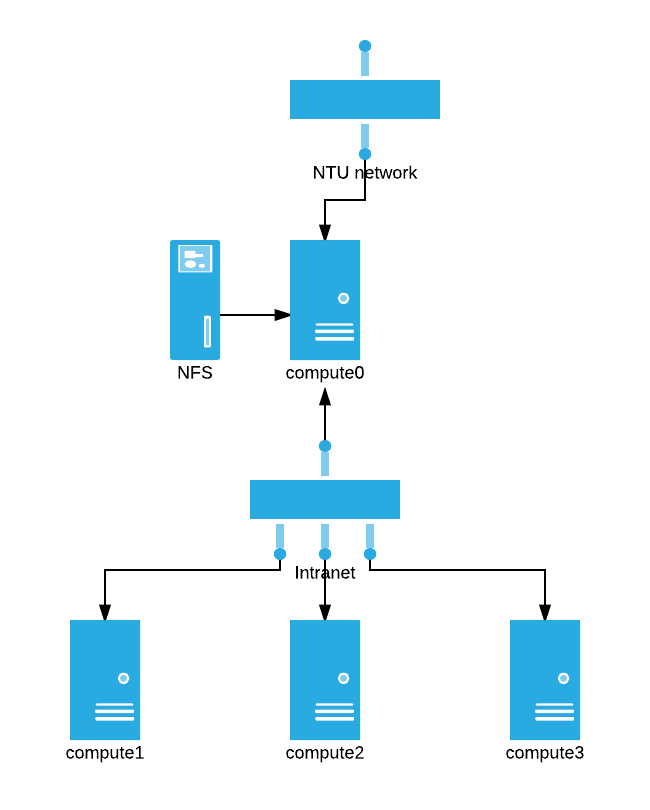
\includegraphics[width=0.55\textwidth]{images/arch.png}
    \caption{NTU HPC cluster architecture}
    \label{fig:arch}
\end{figure}